\documentclass[11pt]{scrartcl}
\usepackage{fullpage}
\usepackage{placeins}


\usepackage{listings} % Coding Syntax coloring
\usepackage{color}
\usepackage{textcomp}
\definecolor{listinggray}{gray}{0.9}
\definecolor{lbcolor}{rgb}{0.9,0.9,0.9}

\usepackage{amsmath}
\usepackage{textcomp}

\lstset{
     backgroundcolor=\color{lbcolor},
     tabsize=4,
     rulecolor=,
     language=matlab,
        basicstyle=\scriptsize,
        upquote=true,
        aboveskip={1.5\baselineskip},
        columns=fixed,
        showstringspaces=false,
        extendedchars=true,
        breaklines=true,
        prebreak = \raisebox{0ex}[0ex][0ex]{\ensuremath{\hookleftarrow}},
        frame=single,
        showtabs=false,
        showspaces=false,
        showstringspaces=false,
        identifierstyle=\ttfamily,
        keywordstyle=\color[rgb]{0,0,1},
        commentstyle=\color[rgb]{0.133,0.545,0.133},
        stringstyle=\color[rgb]{0.627,0.126,0.941},
}
\usepackage{fancyhdr,graphicx,lastpage}% http://ctan.org/pkg/{fancyhdr,graphicx,lastpage}
\fancypagestyle{plain}{
  \fancyhf{}% Clear header/footer
  \fancyhead[R]{
\includegraphics[scale=0.5]{logo.png}}% Right header
  \fancyhead[L]{\textbf{School of Electronic and Electrical Engineering}}
  %\fancyfoot[L]{Name Firstname - v1.0 \\  Date}% Left footer
  \fancyfoot[R]{\thepage\  / \pageref{LastPage}}% Right footer
}
\pagestyle{plain}% Set page style to plain.


\begin{document}
\title{ELEC2430 Matlab Assignment 1}
\subtitle{ Amplitude Modulation System and spectrum analysis}
\author{Yingjie Luan}
\maketitle

\tableofcontents

\section{Laboratory works}
\subsection{performance analysis }
Below is the table of SNR(Signal to Noise ratio) and BER(bit error rate),

\FloatBarrier
\resizebox{\textwidth}{!}{
\begin{tabular}{|l|l|l|l|l|l|l|l|l|l|l|l|}
\hline
1&2&3&4&5&6&7&8&9&10&11&12\\\hline
0.017129&0.008987&0.0040556&0.0015898&0.0004967&0.0001243&2.01e-05&2.2e-06&0&0&0&0\\\hline
\end{tabular}}
\FloatBarrier


\begin{minipage}[t]{\linewidth}
%\label{fig:main}

{
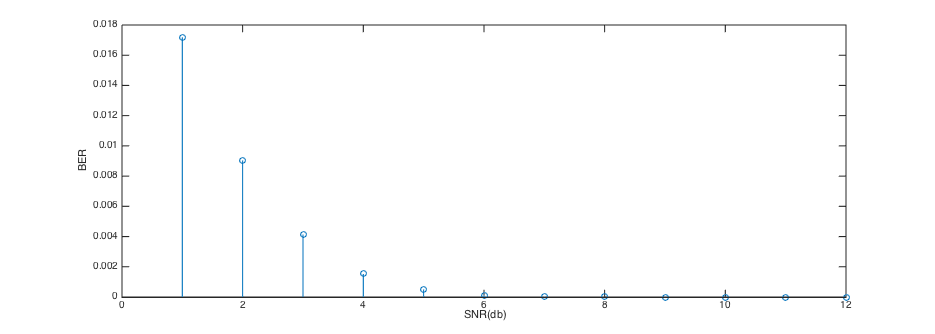
\includegraphics[scale = 0.5]{per.png}
\captionof{figure}{This is the SNR to BER ratio, the BER is decreasing as the noise getting decreased}
}
\end{minipage}
\medskip

Overall, there is 1 million data point for each experiment and it is conducted for 10 times to get the average result.
\subsection{time domain analysis }

\subsubsection{Binary signal}
\begin{minipage}[t]{\linewidth}
%\label{fig:main}

{
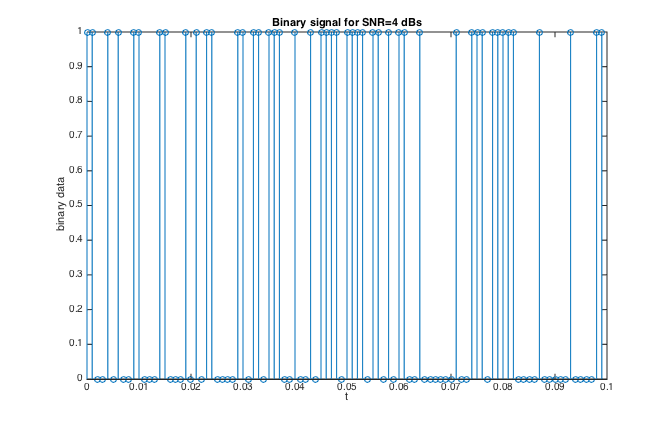
\includegraphics[scale = 0.6]{Binary_signal.png}
\captionof{figure}{This is the first 100 bits of the binary signal.}
}
\end{minipage}
\medskip
\subsubsection{Sampled signal}
\begin{minipage}[t]{\linewidth}
{
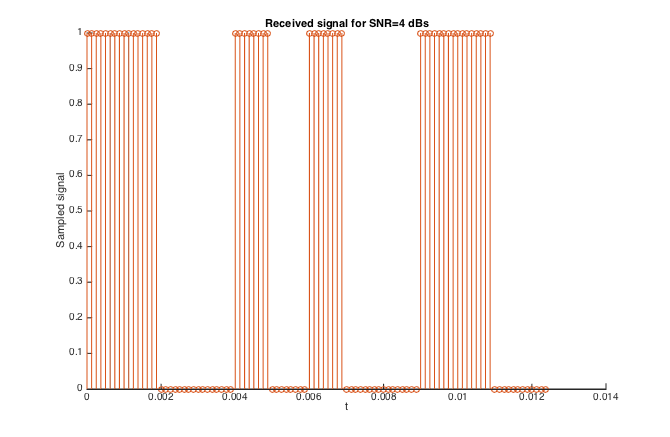
\includegraphics[scale = 0.6]{Sampled_signal.png}
\captionof{figure}{This is the first 100 bits of the sampled signal.}
}
\end{minipage}
\medskip

\subsubsection{Modulated Signal}
\begin{minipage}[t]{\linewidth}
{
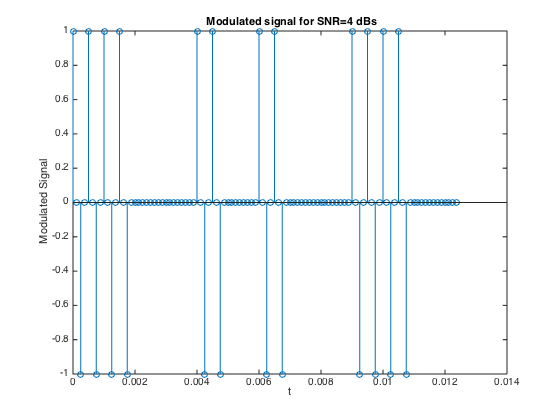
\includegraphics[scale = 0.6]{Modulated_signal.png}
\captionof{figure}{This is the first 100 bits of the modulated signal.}
}
\end{minipage}
\medskip

\subsubsection{Received signal}
\begin{minipage}[t]{\linewidth}
{
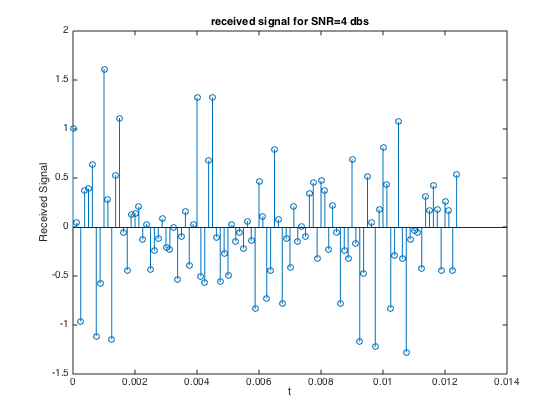
\includegraphics[scale = 0.6]{received_signal.png}
\captionof{figure}{This is the first 100 bits of the received signal.}
}
\end{minipage}
\medskip

\subsubsection{Filtered signal}
\begin{minipage}[t]{\linewidth}
{
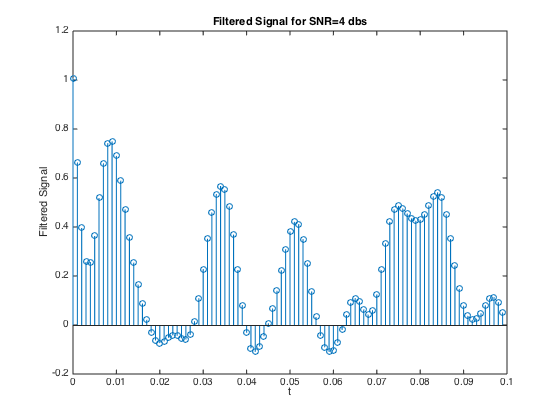
\includegraphics[scale = 0.6]{filtered_signal.png}
\captionof{figure}{This is the first 100 bits of the received signal.}
}
\end{minipage}
\medskip


\subsection{frequency domain analysis }
Below is the required plot, in total, the number of data point is 1 million.
\subsubsection{Filtered signal}
\begin{minipage}[t]{\linewidth}
{
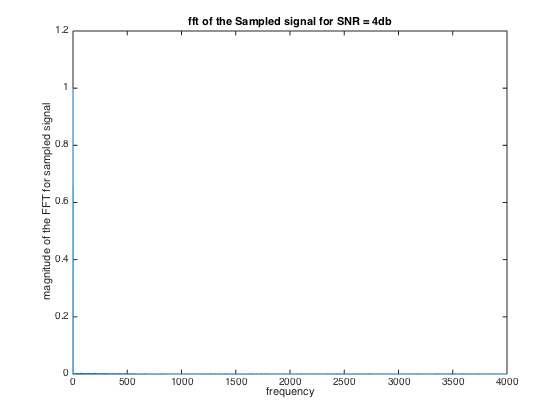
\includegraphics[scale = 0.6]{sampled_signal_fft.png}
\captionof{figure}{This is the of the FFT of the sampled signal.}
}
\end{minipage}
\medskip

\subsubsection{Modulated signal}
\begin{minipage}[t]{\linewidth}
{
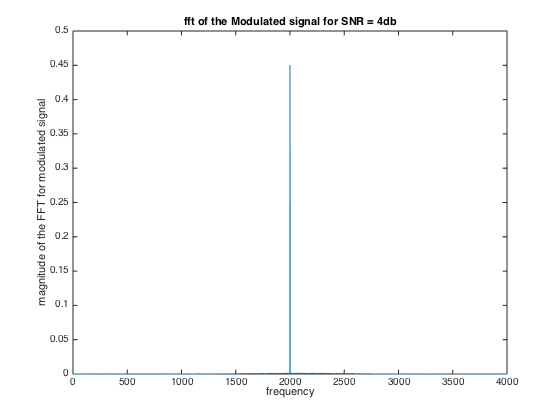
\includegraphics[scale = 0.6]{modulated_signal_fft.png}
\captionof{figure}{This is the of the FFT of the sampled signal.}
}
\end{minipage}
\medskip

\section{Result Analysis}




\end{document}
